% =============================================================================
% pipeline_diagram.tex
% Publication-quality pipeline diagram for:
%   "Comparative Evaluation of Deep Learning Models for
%    Financial Time-Series Forecasting"
%
% Layout: 3-row grid
%   Row 1 – Data Pipeline   : Ingest → Preprocess → Split
%   Row 2 – Training        : HPO → Config Freeze → Final Training
%   Row 3 – Eval & Output   : Aggregation → Benchmarking → Manuscript
%
% Compile with:  pdflatex pipeline_diagram.tex
% Requires: TikZ (standard TeX Live / MiKTeX), no external packages.
% =============================================================================
\documentclass[border=14pt]{standalone}

\usepackage{tikz}
\usepackage{xcolor}
\usepackage{amsmath}
\usepackage{amssymb}
\usepackage[T1]{fontenc}
\usepackage{lmodern}

\usetikzlibrary{
  positioning,
  shapes.geometric,
  arrows.meta,
  backgrounds,
  fit,
  calc,
  patterns
}

% ─────────────────────────────────────────────────────────────────────────────
%  Colour palette
% ─────────────────────────────────────────────────────────────────────────────
\definecolor{dataclr}{RGB}{21,101,192}        % Data – blue
\definecolor{datafill}{RGB}{208,228,248}
\definecolor{hpoclr}{RGB}{194,68,0}           % HPO – burnt-orange
\definecolor{hpofill}{RGB}{255,229,204}
\definecolor{freezeclr}{RGB}{160,108,0}       % Freeze – amber
\definecolor{freezefill}{RGB}{255,248,205}
\definecolor{trainclr}{RGB}{27,140,68}        % Training – green
\definecolor{trainfill}{RGB}{206,246,218}
\definecolor{evalclr}{RGB}{106,44,165}        % Aggregation – purple
\definecolor{evalfill}{RGB}{240,220,255}
\definecolor{statsclr}{RGB}{165,30,30}        % Statistics – dark-red
\definecolor{statsfill}{RGB}{253,215,215}
\definecolor{paperclr}{RGB}{60,80,90}         % Manuscript – slate
\definecolor{paperfill}{RGB}{232,237,240}
% Swim-lane backgrounds
\definecolor{lanedata}{RGB}{239,247,255}
\definecolor{lanetrain}{RGB}{239,252,241}
\definecolor{laneeval}{RGB}{247,239,255}

% ─────────────────────────────────────────────────────────────────────────────
%  Node styles
% ─────────────────────────────────────────────────────────────────────────────
\tikzset{
  %% Main stage boxes  (3.3 cm wide, 1.25 cm tall)
  databox/.style={
    draw=dataclr, fill=datafill, rounded corners=5pt,
    minimum width=3.3cm, minimum height=1.25cm,
    text width=3.1cm, align=center,
    font=\small\bfseries, line width=0.9pt,
  },
  hpobox/.style={
    draw=hpoclr, fill=hpofill, rounded corners=5pt,
    minimum width=3.3cm, minimum height=1.25cm,
    text width=3.1cm, align=center,
    font=\small\bfseries, line width=0.9pt,
  },
  freezebox/.style={
    draw=freezeclr, fill=freezefill, rounded corners=5pt,
    minimum width=3.3cm, minimum height=1.25cm,
    text width=3.1cm, align=center,
    font=\small\bfseries, line width=0.9pt,
  },
  trainbox/.style={
    draw=trainclr, fill=trainfill, rounded corners=5pt,
    minimum width=3.3cm, minimum height=1.25cm,
    text width=3.1cm, align=center,
    font=\small\bfseries, line width=0.9pt,
  },
  evalbox/.style={
    draw=evalclr, fill=evalfill, rounded corners=5pt,
    minimum width=3.3cm, minimum height=1.25cm,
    text width=3.1cm, align=center,
    font=\small\bfseries, line width=0.9pt,
  },
  statsbox/.style={
    draw=statsclr, fill=statsfill, rounded corners=5pt,
    minimum width=3.3cm, minimum height=1.25cm,
    text width=3.1cm, align=center,
    font=\small\bfseries, line width=0.9pt,
  },
  paperbox/.style={
    draw=paperclr, fill=paperfill, rounded corners=5pt,
    minimum width=3.3cm, minimum height=1.25cm,
    text width=3.1cm, align=center,
    font=\small\bfseries, line width=0.9pt,
  },
  %% Sub-annotation boxes (below main nodes)
  subdata/.style={
    draw=dataclr!60, fill=datafill!55, rounded corners=3pt,
    text width=3.1cm, align=left,
    font=\scriptsize, line width=0.5pt,
    inner sep=4pt,
  },
  subhpo/.style={
    draw=hpoclr!60, fill=hpofill!55, rounded corners=3pt,
    text width=3.1cm, align=left,
    font=\scriptsize, line width=0.5pt,
    inner sep=4pt,
  },
  subfreeze/.style={
    draw=freezeclr!60, fill=freezefill!55, rounded corners=3pt,
    text width=3.1cm, align=left,
    font=\scriptsize, line width=0.5pt,
    inner sep=4pt,
  },
  subtrain/.style={
    draw=trainclr!60, fill=trainfill!55, rounded corners=3pt,
    text width=3.1cm, align=left,
    font=\scriptsize, line width=0.5pt,
    inner sep=4pt,
  },
  subeval/.style={
    draw=evalclr!60, fill=evalfill!55, rounded corners=3pt,
    text width=3.1cm, align=left,
    font=\scriptsize, line width=0.5pt,
    inner sep=4pt,
  },
  substats/.style={
    draw=statsclr!60, fill=statsfill!55, rounded corners=3pt,
    text width=3.1cm, align=left,
    font=\scriptsize, line width=0.5pt,
    inner sep=4pt,
  },
  subpaper/.style={
    draw=paperclr!60, fill=paperfill!70, rounded corners=3pt,
    text width=3.1cm, align=left,
    font=\scriptsize, line width=0.5pt,
    inner sep=4pt,
  },
  %% Stage-number badges
  badge/.style={
    circle, minimum size=0.65cm, inner sep=0pt,
    draw=#1!75!black, fill=#1!80, text=white,
    font=\footnotesize\bfseries, line width=0.7pt,
  },
  %% Data-flow arrows (within a row)
  flowarrow/.style={
    ->, >=Latex, line width=1.1pt, color=#1,
    shorten >=2pt, shorten <=2pt,
  },
  %% Row-transition wrap-around arrow (right-end → left-start of next row)
  wraparrow/.style={
    ->, >=Latex, line width=1.1pt, color=#1,
    shorten >=2pt, shorten <=2pt,
    rounded corners=9pt,
  },
  %% Lane header pill (right side of each lane)
  lanelabel/.style={
    rounded corners=4pt,
    draw=#1!45, fill=#1!10,
    inner xsep=6pt, inner ysep=4pt,
    font=\footnotesize\bfseries\sffamily,
    text=#1!80!black,
    align=center,
  },
}

% ─────────────────────────────────────────────────────────────────────────────
%  Helper macro: small bullet item
% ─────────────────────────────────────────────────────────────────────────────
\newcommand{\bul}[1]{\strut\(\cdot\)\hspace{1.5pt}#1\\[0.5pt]}

% ─────────────────────────────────────────────────────────────────────────────
%  Grid coordinates
%    Columns : cA = 0    cB = 5.3    cC = 10.6
%    Rows    : rI = 0    rII = -7.4  rIII = -14.8
% ─────────────────────────────────────────────────────────────────────────────
\def\cA{0}
\def\cB{5.3}
\def\cC{10.6}
\def\rI{0}
\def\rII{-7.4}
\def\rIII{-14.8}

% ═════════════════════════════════════════════════════════════════════════════
\begin{document}
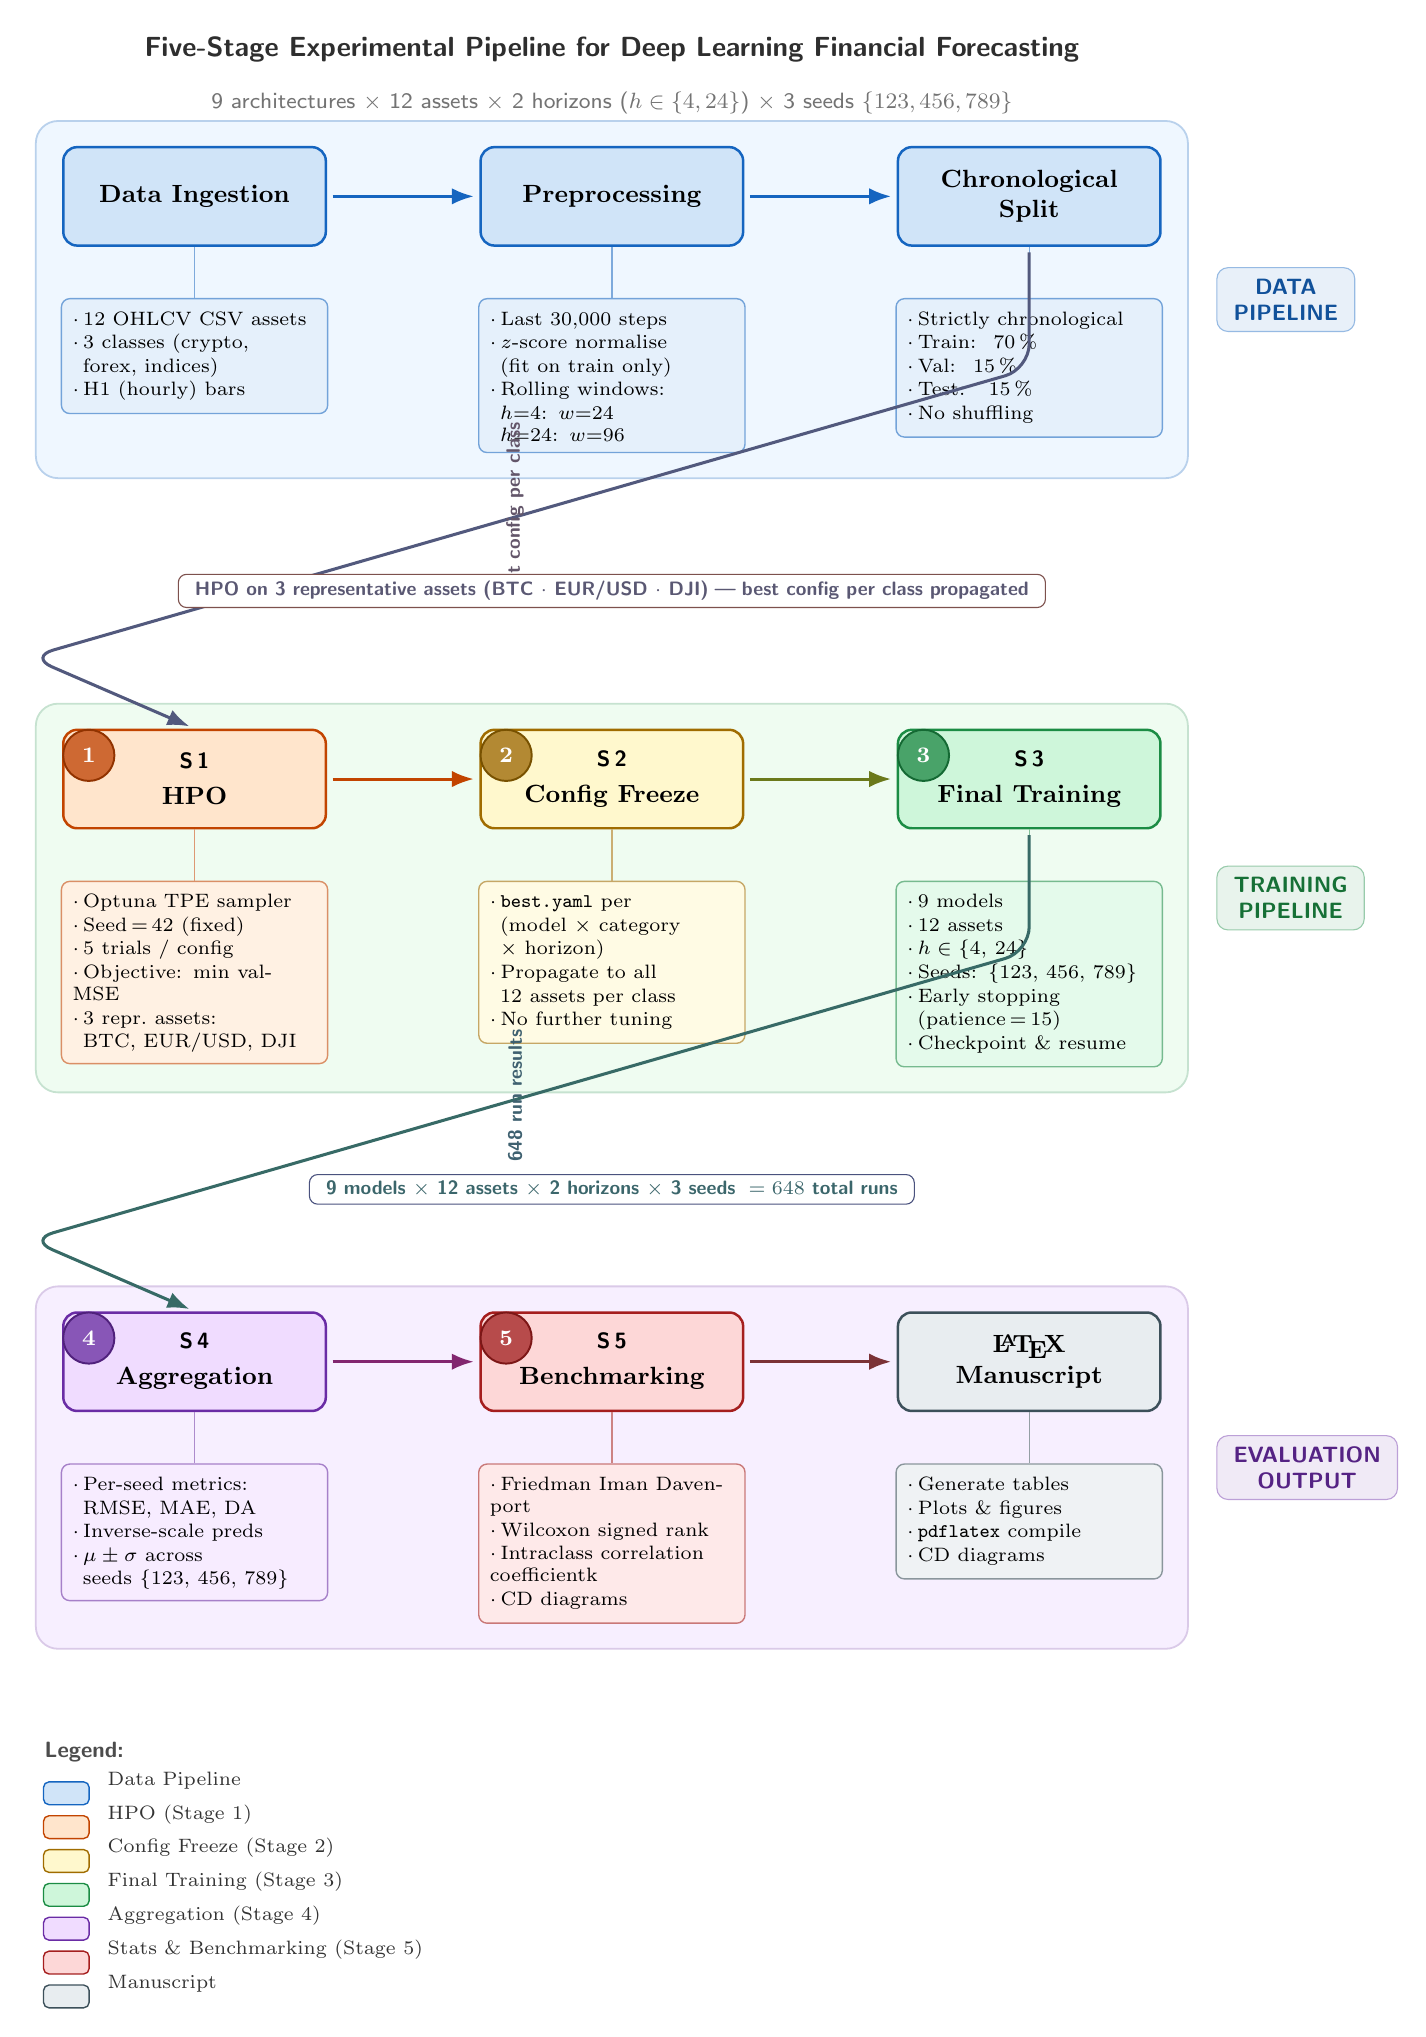
\begin{tikzpicture}[every node/.append style={font=\small}]

% ─────────────────────────────────────────────────────────────────────────────
%  ROW 1 – Data Pipeline
% ─────────────────────────────────────────────────────────────────────────────

\node[databox] (ingest)  at (\cA,\rI) {Data Ingestion};
\node[databox] (preproc) at (\cB,\rI) {Preprocessing};
\node[databox] (split)   at (\cC,\rI) {Chronological\\Split};

% ─────────────────────────────────────────────────────────────────────────────
%  ROW 2 – Training Pipeline
% ─────────────────────────────────────────────────────────────────────────────

\node[hpobox]    (hpo)    at (\cA,\rII) {\textsf{\footnotesize S\,1}\\[2pt]HPO};
\node[freezebox] (freeze) at (\cB,\rII) {\textsf{\footnotesize S\,2}\\[2pt]Config Freeze};
\node[trainbox]  (train)  at (\cC,\rII) {\textsf{\footnotesize S\,3}\\[2pt]Final Training};

% ─────────────────────────────────────────────────────────────────────────────
%  ROW 3 – Evaluation & Output
% ─────────────────────────────────────────────────────────────────────────────

\node[evalbox]  (aggr)  at (\cA,\rIII) {\textsf{\footnotesize S\,4}\\[2pt]Aggregation};
\node[statsbox] (bench) at (\cB,\rIII) {\textsf{\footnotesize S\,5}\\[2pt]Benchmarking};
\node[paperbox] (paper) at (\cC,\rIII) {\LaTeX{}\\Manuscript};


% ─────────────────────────────────────────────────────────────────────────────
%  Sub-annotation boxes  (0.65 cm below each main node)
% ─────────────────────────────────────────────────────────────────────────────

% ── Row 1 ────────────────────────────────────────────────────────────────────
\node[subdata, below=0.65cm of ingest] (sub1) {%
  \bul{12 OHLCV CSV assets}%
  \bul{3 classes (crypto,}%
  \hphantom{\(\cdot\)\,}forex, indices)%
  \\[0.5pt]%
  \bul{H1 (hourly) bars}%
};

\node[subdata, below=0.65cm of preproc] (sub2) {%
  \bul{Last 30{,}000 steps}%
  \bul{$z$-score normalise}%
  \hphantom{\(\cdot\)\,}(fit on train only)%
  \\[0.5pt]%
  \bul{Rolling windows:}%
  \hphantom{\(\cdot\)\,}$h{=}4$: $w{=}24$\\%
  \hphantom{\(\cdot\)\,}$h{=}24$: $w{=}96$%
};

\node[subdata, below=0.65cm of split] (sub3) {%
  \bul{Strictly chronological}%
  \bul{Train:\; 70\,\%}%
  \bul{Val:\; 15\,\%}%
  \bul{Test:\;\; 15\,\%}%
  \bul{No shuffling}%
};

% ── Row 2 ────────────────────────────────────────────────────────────────────
\node[subhpo, below=0.65cm of hpo] (sub4) {%
  \bul{Optuna TPE sampler}%
  \bul{Seed\,=\,42 (fixed)}%
  \bul{5 trials / config}%
  \bul{Objective: $\min$ val-MSE}%
  \bul{3 repr.\ assets:}%
  \hphantom{\(\cdot\)\,}BTC, EUR/USD, DJI%
};

\node[subfreeze, below=0.65cm of freeze] (sub5) {%
  \bul{\texttt{best.yaml} per}%
  \hphantom{\(\cdot\)\,}(model $\times$ category%
  \\[0.5pt]\hphantom{\(\cdot\)\,}$\times$ horizon)%
  \\[0.5pt]%
  \bul{Propagate to all}%
  \hphantom{\(\cdot\)\,}12 assets per class%
  \\[0.5pt]%
  \bul{No further tuning}%
};

\node[subtrain, below=0.65cm of train] (sub6) {%
  \bul{9 models}%
  \bul{12 assets}%
  \bul{$h \in \{4,\,24\}$}%
  \bul{Seeds: \{123, 456, 789\}}%
  \bul{Early stopping}%
  \hphantom{\(\cdot\)\,}(patience\,=\,15)%
  \\[0.5pt]%
  \bul{Checkpoint \& resume}%
};

% ── Row 3 ────────────────────────────────────────────────────────────────────
\node[subeval, below=0.65cm of aggr] (sub7) {%
  \bul{Per-seed metrics:}%
  \hphantom{\(\cdot\)\,}RMSE, MAE, DA%
  \\[0.5pt]%
  \bul{Inverse-scale preds}%
  \bul{$\mu \pm \sigma$ across}%
  \hphantom{\(\cdot\)\,}seeds \{123, 456, 789\}%
};

\node[substats, below=0.65cm of bench] (sub8) {%
  \bul{Friedman Iman Davenport}%
  \bul{Wilcoxon signed rank}%
  \bul{Intraclass correlation coefficientk}%
  \bul{CD diagrams}%
};

\node[subpaper, below=0.65cm of paper] (sub9) {%
  \bul{Generate\ tables}%
  \bul{Plots \& figures}%
  \bul{\texttt{pdflatex} compile}%
  \bul{CD diagrams}%
};


% ─────────────────────────────────────────────────────────────────────────────
%  Stage-number badges  (top-left corner of each stage node)
% ─────────────────────────────────────────────────────────────────────────────

\node[badge=hpoclr,    anchor=center] at ($(hpo.north    west)+(0.34,-0.34)$) {1};
\node[badge=freezeclr, anchor=center] at ($(freeze.north west)+(0.34,-0.34)$) {2};
\node[badge=trainclr,  anchor=center] at ($(train.north  west)+(0.34,-0.34)$) {3};
\node[badge=evalclr,   anchor=center] at ($(aggr.north   west)+(0.34,-0.34)$) {4};
\node[badge=statsclr,  anchor=center] at ($(bench.north  west)+(0.34,-0.34)$) {5};


% ─────────────────────────────────────────────────────────────────────────────
%  Vertical connectors: main node → sub-annotation box
% ─────────────────────────────────────────────────────────────────────────────

\foreach \n/\s/\c in {%
  ingest/sub1/dataclr,%
  preproc/sub2/dataclr,%
  split/sub3/dataclr,%
  hpo/sub4/hpoclr,%
  freeze/sub5/freezeclr,%
  train/sub6/trainclr,%
  aggr/sub7/evalclr,%
  bench/sub8/statsclr,%
  paper/sub9/paperclr%
}{%
  \draw[\c!55, line width=0.45pt] (\n.south) -- (\s.north);
}


% ─────────────────────────────────────────────────────────────────────────────
%  ROW-1 horizontal flow arrows
% ─────────────────────────────────────────────────────────────────────────────

\draw[flowarrow=dataclr] (ingest)  -- (preproc);
\draw[flowarrow=dataclr] (preproc) -- (split);

% ─────────────────────────────────────────────────────────────────────────────
%  ROW-1 → ROW-2  wrap-around connector  (Split → HPO)
%  Path: south of Split → down → hard-left below lane → north of HPO
% ─────────────────────────────────────────────────────────────────────────────

% Intermediate waypoints (chosen to stay in the inter-lane gap)
\coordinate (wrapAB_R) at ($(split.south) + (0,-1.55)$);
\coordinate (wrapAB_L) at (\cA, \rII);
\coordinate (wrapAB_L_above) at ($(\cA, \rII) + (-2.10, 1.55)$);

\draw[wraparrow=dataclr!65!hpoclr]
  (split.south)
  -- (wrapAB_R)
  -- (wrapAB_L_above)
  -- (hpo.north);

% Row-transition label (centred on left spine)
\node[
  font=\scriptsize\sffamily\bfseries,
  text=dataclr!55!hpoclr, rotate=90, anchor=center,
] at ($(wrapAB_L_above)!0.5!(wrapAB_R) + (-0.18,0)$)
  {best config per class};


% ─────────────────────────────────────────────────────────────────────────────
%  ROW-2 horizontal flow arrows
% ─────────────────────────────────────────────────────────────────────────────

\draw[flowarrow=hpoclr]                (hpo)    -- (freeze);
\draw[flowarrow=freezeclr!60!trainclr] (freeze) -- (train);

% ─────────────────────────────────────────────────────────────────────────────
%  ROW-2 → ROW-3  wrap-around connector  (Train → Aggregation)
% ─────────────────────────────────────────────────────────────────────────────

\coordinate (wrapBC_R) at ($(train.south) + (0,-1.55)$);
\coordinate (wrapBC_L_above) at ($(\cA, \rIII) + (-2.10, 1.55)$);

\draw[wraparrow=trainclr!65!evalclr]
  (train.south)
  -- (wrapBC_R)
  -- (wrapBC_L_above)
  -- (aggr.north);

% Row-transition label
\node[
  font=\scriptsize\sffamily\bfseries,
  text=trainclr!55!evalclr, rotate=90, anchor=center,
] at ($(wrapBC_L_above)!0.5!(wrapBC_R) + (-0.18,0)$)
  {648 run results};


% ─────────────────────────────────────────────────────────────────────────────
%  ROW-3 horizontal flow arrows
% ─────────────────────────────────────────────────────────────────────────────

\draw[flowarrow=evalclr!60!statsclr]   (aggr)  -- (bench);
\draw[flowarrow=statsclr!60!paperclr]  (bench) -- (paper);


% ─────────────────────────────────────────────────────────────────────────────
%  Swim-lane background bands  (horizontal, drawn behind everything)
% ─────────────────────────────────────────────────────────────────────────────

\begin{scope}[on background layer]

  % Lane A – Data Pipeline
  \node[
    fill=lanedata, draw=dataclr!30, rounded corners=8pt,
    line width=0.65pt, inner sep=9pt,
    fit=(ingest)(preproc)(split)(sub1)(sub2)(sub3),
  ] (laneA) {};

  % Lane B – Training Pipeline
  \node[
    fill=lanetrain, draw=trainclr!25, rounded corners=8pt,
    line width=0.65pt, inner sep=9pt,
    fit=(hpo)(freeze)(train)(sub4)(sub5)(sub6),
  ] (laneB) {};

  % Lane C – Evaluation & Output
  \node[
    fill=laneeval, draw=evalclr!25, rounded corners=8pt,
    line width=0.65pt, inner sep=9pt,
    fit=(aggr)(bench)(paper)(sub7)(sub8)(sub9),
  ] (laneC) {};

\end{scope}


% ─────────────────────────────────────────────────────────────────────────────
%  Swim-lane header pills (right edge of each lane)
% ─────────────────────────────────────────────────────────────────────────────

\node[lanelabel=dataclr,  anchor=west] at ($(laneA.east)+(0.35,0)$)
  {DATA\\PIPELINE};

\node[lanelabel=trainclr, anchor=west] at ($(laneB.east)+(0.35,0)$)
  {TRAINING\\PIPELINE};

\node[lanelabel=evalclr,  anchor=west] at ($(laneC.east)+(0.35,0)$)
  {EVALUATION\\OUTPUT};


% ─────────────────────────────────────────────────────────────────────────────
%  Inter-lane annotation banners
% ─────────────────────────────────────────────────────────────────────────────

\node[
  draw=dataclr!40!hpoclr, fill=white,
  rounded corners=3pt, inner xsep=6pt, inner ysep=2.5pt,
  font=\scriptsize\bfseries\sffamily,
  text=dataclr!60!hpoclr,
] at ($(laneA.south)!0.5!(laneB.north)$)
  {HPO on 3 representative assets
   (BTC $\cdot$ EUR/USD $\cdot$ DJI)\;—\;best config per class propagated};

\node[
  draw=trainclr!40!evalclr, fill=white,
  rounded corners=3pt, inner xsep=6pt, inner ysep=2.5pt,
  font=\scriptsize\bfseries\sffamily,
  text=trainclr!60!evalclr,
] at ($(laneB.south)!0.5!(laneC.north)$)
  {9 models $\times$ 12 assets $\times$ 2 horizons $\times$ 3 seeds
   \;$= 648$ total runs};


% ─────────────────────────────────────────────────────────────────────────────
%  Legend  (bottom-left, below laneC)
% ─────────────────────────────────────────────────────────────────────────────

\coordinate (legendTL) at ($(laneC.south west)+(0,-1.05)$);

\node[anchor=north west, font=\footnotesize\bfseries\sffamily, text=black!70]
  at (legendTL) {Legend:};

\foreach \idx/\fc/\bc/\lbl in {%
  0/datafill/dataclr/Data Pipeline,%
  1/hpofill/hpoclr/HPO (Stage 1),%
  2/freezefill/freezeclr/Config Freeze (Stage 2),%
  3/trainfill/trainclr/Final Training (Stage 3),%
  4/evalfill/evalclr/Aggregation (Stage 4),%
  5/statsfill/statsclr/Stats \& Benchmarking (Stage 5),%
  6/paperfill/paperclr/Manuscript%
}{%
  \node[
    draw=\bc, fill=\fc, rounded corners=2pt,
    minimum width=0.58cm, minimum height=0.29cm,
    line width=0.5pt, inner sep=0pt, anchor=north west,
  ] at ($(legendTL)+(0.10, -0.62 + \idx*-0.43)$) {};
  \node[anchor=west, font=\scriptsize, text=black!80]
    at ($(legendTL)+(0.80, -0.61 + \idx*-0.43)$) {\lbl};
}


% ─────────────────────────────────────────────────────────────────────────────
%  Title strip  (above laneA)
% ─────────────────────────────────────────────────────────────────────────────

\node[
  anchor=south,
  font=\normalsize\bfseries\sffamily,
  text=black!82,
] at ($(laneA.north)+(0,0.62)$)
  {Five-Stage Experimental Pipeline for Deep Learning Financial Forecasting};

\node[
  anchor=north,
  font=\footnotesize\sffamily,
  text=black!55,
] at ($(laneA.north)+(0,0.48)$)
  {9 architectures $\times$ 12 assets $\times$ 2 horizons
   ($h \in \{4,24\}$) $\times$ 3 seeds~$\{123,456,789\}$};


\end{tikzpicture}
\end{document}

